\documentclass[12pt]{article}

\input preamble

\title{Principles of Parallel Architecture\\
Project Report 3}
\author{Xitong Liu \\
xliu@ece.udel.edu}

\begin{document}

\maketitle

\section{Introduction}
In this report, we will introduce more optimization methods applied
to parallel matrix multiplication. At last, we will report the 
performance in different aspect in detail.

\section{Instruction Level Parallelism}
Instruction level Parallelism (ILP) is one of the most useful techniques 
which can be applied to improve the performance of parallel program 
greatly. In this program, we use gcc to generate the assembly code of 
the method which performs best in methods we proposed in the last 
report. Then we adjust the instructions as well as the instruction 
order to reach the best performance. Several methods were applied:

\begin{enumerate}
\item \textbf{Register Renaming}: reduce the data dependencies between 
the adjacent instructions.
\item \textbf{Instruction Pipelining}: utilize the pipeline of the 
processor to hide the latency of data loading and storing from and to 
the memory.
\item \textbf{Out of Order Execution}: hide the loading and storing 
latency in instructions without data dependency.
\end{enumerate}

During the optimization process, we found some interesting facts from
the assembly code generated by gcc. To our surprise, gcc generates the
instructions in a na\"\i ve way which is inefficient. Here is an example:

\scriptsize
\begin{verbatim}
#oprand_b_0 = __builtin_ia32_loadups(&(matrixBT.data[cycleJ * dim + cycleK]));
	movq	-248(%rbp), %rax
	movq	16(%rax), %rax
	movq	(%rax), %rdx
	movq	-248(%rbp), %rax
	movl	32(%rax), %eax
	imull	-20(%rbp), %eax
	addl	-24(%rbp), %eax
	cltq
	salq	$2, %rax
	leaq	(%rdx,%rax), %rax
	movups	(%rax), %xmm0
	movlps	%xmm0, -192(%rbp)
	movhps	%xmm0, -184(%rbp)       #%xmm0 -> oprand_b_0

#oprand_b_0 = __builtin_ia32_loadups(&(matrixBT.data[(cycleJ  + 1)* dim + cycleK]));
	movq	-248(%rbp), %rax
	movq	16(%rax), %rax
	movq	(%rax), %rdx
	movl	-20(%rbp), %eax
	leal	1(%rax), %ecx
	movq	-248(%rbp), %rax
	movl	32(%rax), %eax
	imull	%ecx, %eax
	addl	-24(%rbp), %eax
	cltq
	salq	$2, %rax
	leaq	(%rdx,%rax), %rax
	movups	(%rax), %xmm0
	movlps	%xmm0, -208(%rbp)
	movhps	%xmm0, -200(%rbp)       #%xmm0 -> oprand_b_1
	
#oprand_b_0 = __builtin_ia32_loadups(&(matrixBT.data[(cycleJ + 2) * dim + cycleK]));
	movq	-248(%rbp), %rax
	movq	16(%rax), %rax
	movq	(%rax), %rdx
	movl	-20(%rbp), %eax
	leal	2(%rax), %ecx
	movq	-248(%rbp), %rax
	movl	32(%rax), %eax
	imull	%ecx, %eax
	addl	-24(%rbp), %eax
	cltq
	salq	$2, %rax
	leaq	(%rdx,%rax), %rax
	movups	(%rax), %xmm0
	movlps	%xmm0, -224(%rbp)
	movhps	%xmm0, -216(%rbp)       #%xmm0 -> oprand_b_2
\end{verbatim}
\normalsize

In this example, the index of the matrix data array is calculated from 
scratch each time to load four numbers to the vector which lead to 
unnecessary and duplicate instruction execution. Actually there is a 
fixed stride (\texttt{dim}) between the indices. So we can calculate 
the index at the first load and increase the index by \texttt{dim} in 
the following loads which may save a lot of instructions. The optimized
code is shown as below:

\scriptsize
\begin{verbatim}
# dim -> %rcx
	movq	-248(%rbp), %rax
	movl	32(%rax), %eax
	cltq
	mov     %rax, %rcx
  
#matrixRT.data -> %rdx
	movq	-248(%rbp), %rax
	movq	16(%rax), %rax
	movq	(%rax), %rdx

#oprand_b_0 = __builtin_ia32_loadups(&(matrixBT.data[cycleJ * dim + cycleK]));
        
# (cycleJ * dim + cycleK) -> %rsi
	movl    %ecx, %eax
	imull	-20(%rbp), %eax         #-20(%rbp) is cycleJ
	addl	-24(%rbp), %eax
	cltq
        
	mov     %rax, %rsi
	add     %rcx, %rsi
	
	salq	$2, %rax
	leaq	(%rdx,%rax), %rax
	movups	(%rax), %xmm0
	movlps	%xmm0, -192(%rbp)
	movhps	%xmm0, -184(%rbp)       #%xmm0 -> oprand_b_0

#oprand_b_1 = __builtin_ia32_loadups(&(matrixBT.data[(cycleJ  + 1)* dim + cycleK]));
	mov     %rsi, %rax
	add     %rcx, %rsi

	salq	$2, %rax
	leaq	(%rdx,%rax), %rax
	movups	(%rax), %xmm0
	movlps	%xmm0, -192(%rbp)
	movhps	%xmm0, -184(%rbp)       #%xmm0 -> oprand_b_0

#oprand_b_2 = __builtin_ia32_loadups(&(matrixBT.data[(cycleJ + 2) * dim + cycleK]));
	mov     %rsi, %rax
	add     %rcx, %rsi

	salq	$2, %rax
	leaq	(%rdx,%rax), %rax
	movups	(%rax), %xmm0
	movlps	%xmm0, -192(%rbp)
	movhps	%xmm0, -184(%rbp)       #%xmm0 -> oprand_b_0
\end{verbatim}
\normalsize

We also found that gcc uses the registers in a very conservative way.
In most cases, gcc only uses \texttt{xmm0} and \texttt{xmm1}, while
there are 16 \texttt{xmm} registers in total. See the following example:

\scriptsize
\begin{verbatim}
#acc_0 = __builtin_ia32_addps(acc_0, __builtin_ia32_mulps(oprand_a, oprand_b_0));
	xorps	%xmm0, %xmm0
	movlps	-192(%rbp), %xmm0
	movhps	-184(%rbp), %xmm0
	xorps	%xmm1, %xmm1
	movlps	-176(%rbp), %xmm1
	movhps	-168(%rbp), %xmm1
	mulps	%xmm1, %xmm0
	addps	-48(%rbp), %xmm0
	movlps	%xmm0, -48(%rbp)
	movhps	%xmm0, -40(%rbp)

#acc_1 = __builtin_ia32_addps(acc_0, __builtin_ia32_mulps(oprand_a, oprand_b_1));
	xorps	%xmm0, %xmm0
	movlps	-208(%rbp), %xmm0
	movhps	-200(%rbp), %xmm0
	xorps	%xmm1, %xmm1
	movlps	-176(%rbp), %xmm1
	movhps	-168(%rbp), %xmm1
	mulps	%xmm1, %xmm0
	addps	-64(%rbp), %xmm0
	movlps	%xmm0, -64(%rbp)
	movhps	%xmm0, -56(%rbp)

#acc_2 = __builtin_ia32_addps(acc_0, __builtin_ia32_mulps(oprand_a, oprand_b_2));
	xorps	%xmm0, %xmm0
	movlps	-224(%rbp), %xmm0
	movhps	-216(%rbp), %xmm0
	xorps	%xmm1, %xmm1
	movlps	-176(%rbp), %xmm1
	movhps	-168(%rbp), %xmm1
	mulps	%xmm1, %xmm0
	addps	-80(%rbp), %xmm0
	movlps	%xmm0, -80(%rbp)
	movhps	%xmm0, -72(%rbp)

#acc_3 = __builtin_ia32_addps(acc_0, __builtin_ia32_mulps(oprand_a, oprand_b_3));
	xorps	%xmm0, %xmm0
	movlps	-240(%rbp), %xmm0
	movhps	-232(%rbp), %xmm0
	xorps	%xmm1, %xmm1
	movlps	-176(%rbp), %xmm1
	movhps	-168(%rbp), %xmm1
	mulps	%xmm1, %xmm0
	addps	-96(%rbp), %xmm0
	movlps	%xmm0, -96(%rbp)
	movhps	%xmm0, -88(%rbp)
\end{verbatim}
\normalsize

Obviously gcc only use gcc only uses \texttt{xmm0} and \texttt{xmm1}
for SSE instructions and other variables are stored in memory. Each
time it loads data from memory to \texttt{xmm} register, do the 
calculation( multiplication, addition ) and stores data from 
\texttt{xmm} register to memory, which is far beyond our expectation.
After the optimization, each intermediate vector variable 
(\texttt{acc\_0}, \texttt{acc\_1}, \texttt{oprand\_b\_0}, 
\texttt{oprand\_b\_1} etc.) were bind to dedicated \texttt{xmm} 
registers and the data exchanges between memory and registers 
were saved greatly.

\scriptsize
\begin{verbatim}
#register map
#xmm0 xmm1 xmm2 reserved for arithmetic operation
#xmm3 oprand_a
#xmm4 acc_0
#xmm5 acc_1
#xmm6 acc_2
#xmm7 acc_3
#xmm8 oprand_b_0
#xmm9 oprand_b_1
#xmm10 oprand_b_2
#xmm11 oprand_b_3

#acc_0 = __builtin_ia32_addps(acc_0, __builtin_ia32_mulps(oprand_a, oprand_b_0));
movups  %xmm3, %xmm12
movups  %xmm3, %xmm13
movups  %xmm3, %xmm14
movups  %xmm3, %xmm15

mulps   %xmm8, %xmm12
mulps   %xmm9, %xmm13
mulps   %xmm10, %xmm14
mulps   %xmm11, %xmm15

addps   %xmm12, %xmm4

#acc_1 = __builtin_ia32_addps(acc_0, __builtin_ia32_mulps(oprand_a, oprand_b_1));
addps   %xmm13, %xmm5

#acc_2 = __builtin_ia32_addps(acc_0, __builtin_ia32_mulps(oprand_a, oprand_b_2));
addps   %xmm14, %xmm6

#acc_3 = __builtin_ia32_addps(acc_0, __builtin_ia32_mulps(oprand_a, oprand_b_3));
addps   %xmm15, %xmm7
\end{verbatim}
\normalsize

In the above optimized code, the calculation was fully pipelined.

\section{Experiment Results}
\subsection{Overall Performance}
We measure the execution time of different methods under different matrix sizes,
and calculate the \textsc{SpeedUp} in the following way:
\begin{equation}
\textsc{SpeedUp} = \frac{T_{serial}}{T_{parallel}}
\end{equation}
The results were shown as below:

\begin{figure}[h!]
	\begin{center}
		\includegraphics[width=1.0\textwidth, angle=0]{performance.png}
		\caption{\label{fig:performance}Performance comparision}
	\end{center}
\end{figure}

Obviously ILP outperforms other methods. The greatest \textsc{SpeedUp} was 91.03,
reached with ILP when the matrix size is 1024. When the matrix size was small, 
the performance was limited by the overhead of threads startup and synchronization
when the threads exit. When the matrix size was larger than 1024, the performance
decreased since cache misses and invalidation increased dramatically.

\subsection{MFLOPS}
The MFLOPS with different matrix sizes was measured with 32 threads, shown in 
Figure~\ref{fig:mflops}. MFLOPS reaches maximum when the matrix size is between
256 and 1024. As the matrix size increases, the MFLOPS decrease as cache misses
increase.
\begin{figure}[h!]
	\begin{center}
		\includegraphics[width=.7\textwidth, angle=0]{mflops.png}
		\caption{\label{fig:mflops}MFLOPS with different matrix sizes}
	\end{center}
\end{figure}

\subsection{Cache Miss}
The L2 Cache Miss with different matrix sizes was measured with 32 threads, 
shown in Figure~\ref{fig:l2cachemiss}. Intuitively the L2 cache misses increase
as matrix size increases. We found an interesting fact that when the matrix size
increases from 1792 to 2048, the L2 cache miss increased dramatically for the 
baseline method ( in which matrix transpose was not applied ). We infer that 
2048 in the threshold. Once passed the threshold, the calculation of each element 
in matrix $\mathbf{C}$ will cause the invalidation of each cache line which is 
a great hazard to the performance. After the transpose of matrix $\mathbf{B}$ 
is applied, we see the decrease of L2 cache misses.

\begin{figure}[h!]
	\begin{center}
		\includegraphics[width=.7\textwidth, angle=0]{l2cachemiss.png}
		\caption{\label{fig:l2cachemiss}L2 cache misses with different matrix sizes}
	\end{center}
\end{figure}

\section{Conclusion}

\end{document}

\begin{comment}
\begin{figure}[h!]
	\begin{center}
		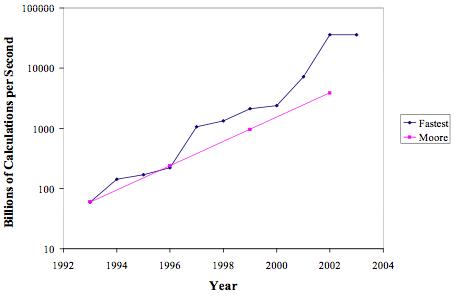
\includegraphics[width=0.7\textwidth, angle=0]{fatest.png}
		\caption{\label{fig:fatest}Fatest SuperComputer in the world}
	\end{center}
\end{figure}
\end{comment}